% - starred version (e.g. \section*{Section name}) disables the (sub)section page.

\documentclass[czech]{beamer}
\usepackage{babel}

\usepackage{fontawesome5}

% use the focus theme (without fira)
\usetheme[nofirafonts]{focus}
\usefonttheme{serif}

% shamelessly stolen from https://www.patrickbaylis.com/posts/2018-10-11-beamer-resizing/
\usepackage{adjustbox}
\makeatletter
\newcommand{\fitimage}[2][\@nil]{
	\begin{figure}
		\begin{adjustbox}{width=0.9\textwidth, totalheight=\textheight-2\baselineskip-2\baselineskip,keepaspectratio}
			\includegraphics{#2}
		\end{adjustbox}
		\def\tmp{#1}%
	 \ifx\tmp\@nnil
			\else
			\caption{#1}
		\fi
	\end{figure}
}
\makeatother

\setlength{\belowcaptionskip}{-7pt}

% bullets
\setbeamertemplate{itemize item}{$\bullet$}
\setbeamertemplate{itemize subitem}{$\bullet$}
\setbeamertemplate{itemize subsubitem}{$\bullet$}
\setbeamercolor{itemize subsubitem}{fg=main}

% code
\usepackage{minted}
\setminted[python]{
	linenos,
	mathescape=true,
	escapeinside=||,
	autogobble,
	obeytabs=true,
	tabsize=4}

% strikethrough
\usepackage{soul}

% tables
\usepackage{booktabs}

% number lemmas and theorems
\setbeamertemplate{theorems}[numbered]

\makeatletter
\AtBeginEnvironment{proof}{\let\@addpunct\@gobble}
\makeatother

% translations
\newtranslation[to=Czech]{Definition}{Definice}


\title{In-place BFS a DFS}
\subtitle{v lineárním čase na modelu RAM}
\date{Tomáš Sláma \hfill 7. 4. 2020}

\begin{document}
	\begin{frame}
		\maketitle
	\end{frame}
	
	\section{Úvod}
	\begin{frame}{Předpoklady}
		\begin{itemize}
			\item pracujeme s modelem RAM
			\begin{itemize}
				\item paměť je pole slov velikosti $w$
				\item operace se slovy (čtení, psaní, přístupy) jsou konstantní
				\item vstup je na prvních $n \in \mathbb{N}$ slovech
				\item velikost $w = \Omega\left(\log n\right)$
			\end{itemize}
			\vfill
			\item \textbf{restore model:} vstup může být měněn v průběhu výpočtu, ale na jeho konci musí být v původním stavu
			\vfill
			\item graf je zadán v setříděném seznamu sousedů
		\end{itemize}

		\fitimage[setřízená reprezentace]{images/sorted.png}
	\end{frame}

	\section{DFS}

	\begin{frame}{Přehled}
		\begin{enumerate}
			\item graf převedeme do speciální reprezentace
			\item budeme v ní kódovat stav DFS (a trochu ji tím rozbijeme)
			\item obnovíme původní stav
			\item převedeme zpět do setřízené reprezentace
		\end{enumerate}
	\end{frame}

	\begin{frame}{Disclaimer}
		\begin{table}
			\centering
			\begin{tabular}{llc}
				\toprule
				\emph{operace} & \emph{význam} & \emph{podpora} \\
				\midrule
				\mintinline{python}{pre-process} & po vstoupení do vrcholu & $\checkmark$ \\
				\mintinline{python}{pre-explore} & po iteraci přes souseda &  \\
				\mintinline{python}{post-process} & po zpracovaní všech sousedů & $\checkmark$ \\
				\mintinline{python}{post-explore} & po vrácení z vrcholu &  \\
				\bottomrule
			\end{tabular}
			\caption{podporované funkce DFS}
		\end{table}
	\end{frame}

	\begin{frame}{Reprezentace}
		\fitimage{images/sorted.png}
		\fitimage{images/pointer.png}
		\fitimage[setřízená, pointerová a prohozená reprezentace]{images/swapped.png}
		\begin{itemize}
			\item pozor na stupně $0$ (zachovávají si jména vrcholů)!
		\end{itemize}
	\end{frame}

	\begin{frame}{setřízená $\rightarrow$ pointerová}
		\begin{lemma}
			Setříděná reprezentace jde do pointerové reprezentace převést in-place v čase $\mathcal{O}\left(n\right)$.
		\end{lemma}

		\begin{proof}
			Nastavíme $A[i] = T\left[A\left[i\right]\right] \forall i \in \left\{n + 2, \ldots, n + m + 2\right\}$ \\
			a $T\left[v\right] = v$ (pro vrcholy $v$ stupně $0$).
		\end{proof}
	\end{frame}

	\begin{frame}{pointerová $\longleftrightarrow$ prohozená}
		\begin{lemma}
			Pointerová jde do prohozené reprezentace (a zpět) převést in-place v čase $\mathcal{O}\left(n\right)$.
		\end{lemma}

		\begin{proof}
			Převod $\rightarrow$: $$T[i] = A[T[i]]\ \text{a}\ A[T[i]] = i\quad \forall i \in \left\{1, \ldots, n\right\}, i \neq T[i]$$
			Převod $\leftarrow$: $$T[A[i]] = i\ \text{a}\ T[A[i]] = i \quad \forall i \in \left\{n + 2, \ldots, n + m + 2\right\}, A[i] < n$$
		\end{proof}
	\end{frame}

	\begin{frame}{prohozená $\rightarrow$ setřízená}
		\begin{lemma}
			Prohozená jde do setřízené reprezentace převést in-place v čase $\mathcal{O}\left(n\right)$.
		\end{lemma}
	\end{frame}

	\begin{frame}{prohozená $\rightarrow$ setřízená}
		\begin{proof}[Důkaz]
			\small
			Nejprve nastavíme 
			\begin{gather*}
				A[i] = A[A[i]]\ \forall i \in \left\{n + 2, \ldots, n + m + 2\right\}, A[i] > n \\
				\text{a} \\
				T[i] = A[T[i]]\ \forall i \in \left\{1, \ldots, n\right\}
			\end{gather*}

			Pak postupně hledáme jména vrcholů $v$ na pozicích $p$ v každém poli sousednosti a nastavujeme:
			$$A[p] = T[v]\ \text{a}\ T\left[v\right] = p$$

			Nakonec opravíme vrcholy stupně $0$ procházením $T$ a nastavením
			$$T[i] = T[i - 1]\ \forall i \in \left\{1, \ldots, n\right\}, T[i] = i$$
		\end{proof}
	\end{frame}

	\begin{frame}{prohozená $\rightarrow$ setřízená}
	\begin{itemize}
			\item důkaz z článku je problematický\footnote{Pokud jsem ho tedy pochopil správně :).}, jelikož nepoznáme, když procházíme nové pole sousednosti
		\end{itemize}
		\fitimage[problematický případ]{images/sorted-pointer-problem.png}
		\begin{proof}[Důkaz (fix)]
			Při nalezení chybného prohození iterujeme o rozdíl správného $v$ s aktuálním a prohazujeme zpět.
		\end{proof}
	\end{frame}

	\subsection{Vrcholy se stupněm $\ge 2$}

	\begin{frame}{Zavedení invariantu}
		\begin{block}{Invariant}
			Vrchol $v$ je bílý $\iff A[T[v]] \le n$.
		\end{block}
		\begin{itemize}
			\item stav vrcholů budeme udržovat přes invariant
			\item na začátku platí pro všechny vrcholy
		\end{itemize}
		\vfill
		\fitimage[prohozená reprezentace]{images/swapped.png}
	\end{frame}

	\begin{frame}{Procházení přes obrácené pointery}
		\begin{itemize}
			\item jsme ve vrcholu $u$ a iterujeme přes jeho sousedy
			\item na pozici $p$ jsme narazili na pointer $q$ do bílého vrcholu $v$, jehož nejmenší soused je na pozici $q'$
			\item nastavíme $T[v] = p$ a $A[p] = q'$
		\end{itemize}
		\fitimage[diagram konstrukce obráceného pointeru]{images/deg2.png}
		\begin{itemize}
			\item pozorování: vrchol $v$ už není bílý
		\end{itemize}
	\end{frame}

	\begin{frame}{Problémy s obrácenými pointery}
		\begin{itemize}
			\item na pozici $p$ uvažujeme první hranu vrcholu $u$ (uložená na $A[T[u]]$) směřující do $v$: kam nasměrovat obrácený pointer?
			\begin{enumerate}
				\item uložit do $A[p]$ -- ztratíme pojem o tom, kde $u$ začíná
				\item uložit do $T[u]$ -- tam už je obrácený pointer
			\end{enumerate}
			\item problém vyřešíme tím, že ho nebudeme řešit:
			\begin{itemize}
				\item pokud by měl nastat, tak prohodíme $T[u]$ s $A[p + 1]$
				\item jelikož jsou pointery setřízené, tak prohození poznáme
			\end{itemize}
			\vfill
		\end{itemize}
		\fitimage[problémy a řešení konstrukce prohozeného pointeru]{images/reverse-pointer-problems.png}
	\end{frame}

	\begin{frame}{Backtrackování}
		\begin{itemize}
			\item po prozkoumání sousedů $v$ narazíme na pozici $q''$ na vrchol $v''$
			\begin{itemize}
				\item poznáme tak, že $A[q''] \le n$
			\end{itemize}
			\item iterujeme zpět do té doby, než $A[p] \le n$
		\end{itemize}

		\begin{figure}
			\centering
			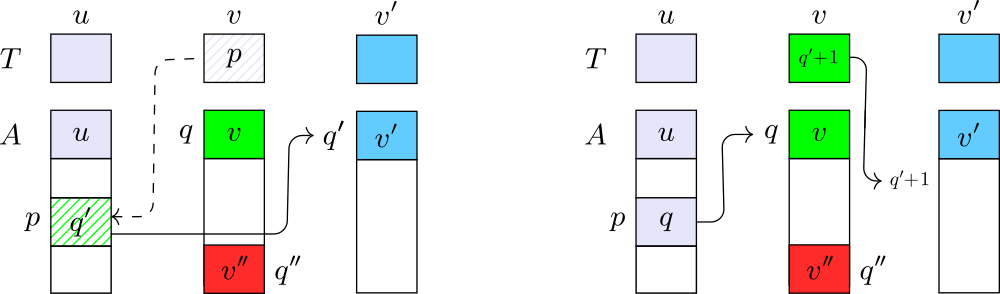
\includegraphics{images/deg2-fix.png}
			\caption{backtrackování}
		\end{figure}
		\begin{itemize}
			\item problém: vrchol $v$ už je zase bílý
			\begin{itemize}
				\item fix: $q' = q' + 1$ -- jelikož jsou stupně všech vrcholů $\ge 2$, tak po inkrementu $q'$ ukazuje na nějaký pointer
			\end{itemize}
		\end{itemize}
	\end{frame}
		
	\subsection{Průběh algoritmu}

	\begin{frame}{Invarianty před a po follow/backtrack}
		\begin{enumerate}
				\item Vrchol $v$ je bílý $\iff$ není startovní a $1 \le A[T[v]] \le n$
				\item Každý šedočerný vrchol (kromě startovního) na aktuální DFS cestě si ukládá obrácený pointer na pozici $T[v]$, která ukazuje, kde byl pointer na $v$ původně uložen v poli sousednosti svého rodiče.
				\item První pointer aktuálně neprocházeného šedočerného vrcholu $v$ (uložený v $T[v]$), ukazuje na druhou pozici pole sousedů nějakého vrcholu.
		\end{enumerate}
	\end{frame}

	\begin{frame}{\st{Pseudokód} Python}
		\begin{center}
			\href{run:presentation.py}{\faPython\ presentation.py} 
		\end{center}
	\end{frame}

	\subsection{Vrcholy se stupněm $0$}

	\begin{frame}{Rozšíření invariantu}
		\begin{block}{Invariant}
			Vrchol $v$ je bílý $\iff A[T[v]] \le n \lor T\left[v\right] = v$.
		\end{block}
		\begin{minipage}[t]{0.5\textwidth}
				\vspace{0pt}
				\begin{itemize}
					\item chováme se normálně
				\end{itemize}
				\fitimage{images/deg0-2.png}
		\end{minipage}%
		\hfill
		\begin{minipage}[t]{0.5\textwidth}
			\vspace{0pt}
			\begin{itemize}
				\item vytvoříme pointer do $T[u]$
			\end{itemize}
			\fitimage{images/deg0-1.png}
		\end{minipage}
		\vfill
		\begin{itemize}
			\item na rozdíl od vrcholů stupně $2$ po sobě neuklízíme
			\begin{itemize}
				\item vlastně vytváříme smyčky (bude se hodit při obnovení)
			\end{itemize}
		\end{itemize}
	\end{frame}

	\subsection{Vrcholy se stupněm $1$}
	\begin{frame}{Dokončení invariantu}
		\begin{block}{Invariant}
			Vrchol $v$ je bílý $\iff (\underbrace{T\left[v\right] = v}_{\text{stupeň}\ 0} \lor \underbrace{T[v] > n}_{\text{stupeň}\ 1, 2}) \land \underbrace{A[T[v]] \le n}_{\text{stupeň}\ \ge2}$.
		\end{block}
		\vfill
		\begin{itemize}
			\item z vrcholu $u$ stupně $\ge 2$ navštívíme bílý vrchol $v$ stupně $1$
			\item podle stupně jediného souseda $v'$ vrcholu $v$ se chováme různě:
			\begin{enumerate}
				\item[0)] jako jsme popisovali výše
				\item[1)] nastavíme $T[v'] = v$ a pokračujeme
				\item[$\ge 2$)] nastavíme $A[\overline{p}] = T[v'']$ a $T[v''] = v'$
			\end{enumerate}
		\end{itemize}
		\fitimage{images/deg1.png}
	\end{frame}

	\subsection{Obnovení}
	\begin{frame}{Obnovení}
		\hfill
		\begin{minipage}[t]{0.97\textwidth}
			\begin{enumerate}
				\item[$\ge 2$)] stačí nastavit $T[v] = T[v] - 1$
				\item[0)] tvoří smyčku, nebo ukazuje na druhou pozici vrcholu:
				\begin{itemize}
					\item iterujeme přes pole sousednosti a hledáme $v = A[p]: v \le n$:
					\begin{itemize}
						\item $T[v] = p$ (smyčka, stupeň $2$)
						\item $T[v] \le n \land T[T[v]] = p + 1$ (prohozený $1$ a $2$ vrchol, stupeň $2$)
						\item $T[v] \le n \land T[T[v]] = v$ (stupeň $1$)
					\end{itemize}
				\end{itemize}
				\item[1)] postupně hledáme vrcholy $v'$ stupně $1$
				\begin{itemize}
					\item pokud ještě nebyly opraveny, obracíme prohozené pointery
				\end{itemize}
			\end{enumerate}
		\end{minipage}
	\end{frame}

	\section{BFS}
	\begin{frame}{Přehled}
		\begin{enumerate}
			\item graf získáme v setřízené reprezentaci
			\item $T$ zkomprimujeme na $\mathcal{T}$ s tím, že:
			\begin{itemize}
				\item zachováme konstantní přístup
				\item uvolníme lineární počet bitů
			\end{itemize}
			\item uvolněné místo použijeme na datovou strukturu pro ukládání stavů vrcholů
			\item provedeme BFS
			\item $\mathcal{T}$ dekomprimujeme na $T$, čímž obnovíme původní stav
		\end{enumerate}
	\end{frame}

	\begin{frame}{Color choice dictionary}
		\begin{itemize}
			\item zobecnění struktury choice dictionary
			\item udřuje $S_0, \ldots, S_{c - 1}$ podmnožin $\left\{1, \ldots, n\right\}$, kde:

				$$\bigcap_{i=0}^{c-1} S_i = \emptyset \qquad\bigcup_{i=0}^{c-1} S_i = \left\{1, \ldots, n\right\}$$

			\item vyžaduje řádově $nc$ bitů paměti
		\end{itemize}

		\vfill

		\begin{table}
			\centering
			\begin{tabular}{llc}
				\toprule
				operace & význam & složitost \\
				\midrule
				\mintinline{python}{setColor(v, c)} & nastaví barvu $v$ na $c$        & $\mathcal{O}\left(1\right)$ \\
				\mintinline{python}{getColor(v)}    & získá barvu $v$                 & $\mathcal{O}\left(1\right)$ \\
				\mintinline{python}{choice(c)}      & získá libovolný $v$ s barvu $c$ & $\mathcal{O}\left(1\right)$ \\
				\bottomrule
			\end{tabular}
			\caption{podporované operace CCD}
		\end{table}
	\end{frame}

	\begin{frame}{Komprimace $T$}
		\begin{itemize}
			\item potřebujeme uvolnit $nc$ bitů
				\vfill
			\item najdeme pozice, kde se mění $c + 1$ MSbitů ve slovech z $T$
			\begin{itemize}
				\item díky setříděnosti jich bude právě $2^{c - 1}$
				\item každé slovo o tolik bitů zkrátíme
				\item zapamatujeme si pozice změn v $T$
			\end{itemize}
				\vfill
			\item dohromady $nw - n(w - (c + 1)) = n(c + 1) = nc + n$
			\begin{itemize}
				\item omezení: $n \ge 2^{c - 1}w$, abychom mohli uložit pozice
			\end{itemize}
		\end{itemize}

		\fitimage[komprimovaná reprezentace $\mathcal{T}$]{images/compression.png}
	\end{frame}

	\begin{frame}{Získávání hodnot z $\mathcal{T}$}
		\begin{enumerate}
			\item bitovými operacemi získáme $w - (c + 1)$ LSbitů slova
			\begin{itemize}
				\item $i$-té slovo v $\mathcal{T}$ začíná na pozici $(w - (c + 1))(i - 1)$
			\end{itemize}
			\item procházíme postupně $2^{c - 1}$ pozic, podle kterých zrekonstruujeme $c + 1$ MSbitů
		\end{enumerate}
	\end{frame}


	\begin{frame}[fragile]{Průběh BFS}
		\small
		\begin{minted}[xleftmargin=.08\textwidth]{python}
			D = ColorChoiceDictionary(WHITE, LIGHT, DARK, BLACK)
			D.setColor(start, LIGHT)

			while choice(LIGHT) is not None:
				while choice(LIGHT) is not None:
					v = D.choice(LIGHT)  # pop node

					# open all white neighbours
					for i in range(|$\mathcal{T}[v]$|, |$\mathcal{T}[v + 1]$|):
						if D.getColor(|$A[i]$|) is WHITE:
							D.setColor(|$A[i]$|, DARK)

					D.setColor(v, BLACK)  # close the node

				LIGHT, DARK = DARK, LIGHT  # next round
		\end{minted}
	\end{frame}

	\begin{frame}[focus]
		Díky za pozornost!
	\end{frame}
	
	\appendix
	\begin{frame}{Zdroje a dodatečné materiály}
		\nocite{*}
		\bibliography{presentation}
		\bibliographystyle{plain}
	\end{frame}
\end{document}
